\section{Anwendungsfälle}
Aus den in Kapitel \ref{chap:szenarien} erarbeiteten Szenarien ergeben sich die folgenden Use-Cases, die von einer offlinefähigen Anwendung erfüllt werden sollen.
\begin{table}[H]
\centering \small
  \begin{tabular}{@{}>{\columncolor[HTML]{cffcc2}}l ll@{} p{0.1\textwidth}p{0.4\textwidth}p{0.4\textwidth}} \toprule
\multicolumn{1}{c}{\cellcolor[HTML]{cffcc2}\textbf{ID}}
& \multicolumn{1}{c}{\cellcolor[HTML]{cffcc2}\textbf{Anwendungsfall}}
& \multicolumn{1}{c}{\cellcolor[HTML]{cffcc2}\textbf{Beschreibung}} \\
\hline
% UC1
\multicolumn{1}{l}{\cellcolor[HTML]{cffcc2}\textbf{UC1}} & \multicolumn{1}{p{0.45\textwidth}}
{Um die Anwendung auch ohne Internetzugang zu nutzen, sollen die Daten auch offline erreichbar sein.}
& \multicolumn{1}{p{0.45\textwidth}}
{Die Daten werden auf dem Server und lokal gespeichert. Lokal bedeutet in einer lokalen Datenbank oder im Browser (localStorage, IndexedDB usw.)}.\\
\midrule
% UC2
\multicolumn{1}{l}{\cellcolor[HTML]{cffcc2}\textbf{UC2}} & \multicolumn{1}{p{0.45\textwidth}}
{Um Datentraffic und Ladezeiten zu sparen möchte ich nur die Adressbucheinträge laden, die sich nicht schon auf dem Endgerät befinden. \todo{Aktualisierungen}}
& \multicolumn{1}{p{0.45\textwidth}}
{Es wird ermittelt welche Daten neu angelegt oder aktualisiert wurden. Dazu müssen sie sortierbar und versionierbar sein.}\\
\midrule
% UC3
\multicolumn{1}{l}{\cellcolor[HTML]{cffcc2}\textbf{UC3}} & \multicolumn{1}{p{0.45\textwidth}}
{Um jedem Adressbucheintrag Operationen zuzuweisen, möchte ich die Einträge identifizieren.}
& \multicolumn{1}{p{0.45\textwidth}}
{Jeder Eintrag bekommt zur eindeutigen Identifikation eine \gls{UUID} zugewiesen.}\\
\midrule
% UC4
\multicolumn{1}{l}{\cellcolor[HTML]{cffcc2}\textbf{UC4}} & \multicolumn{1}{p{0.45\textwidth}}
{Um zu wissen ob, wie oft und wann ein Eintrag aktualisiert wurde, möchte ich die Einträge versionieren.}
& \multicolumn{1}{p{0.45\textwidth}}
{\todo{Jeder Eintrag bekommt eine geordnete Liste von inhaltsbasierten Versionen.}}\\
\midrule
% UC5
\multicolumn{1}{l}{\cellcolor[HTML]{cffcc2}\textbf{UC5}} & \multicolumn{1}{p{0.45\textwidth}}
{Um sicherzustellen, dass keine Daten verloren gehen, soll mit Konflikten umgegangen werden.}
& \multicolumn{1}{p{0.45\textwidth}}
{\todo{Jeder Konflikt wird (in der Versionsliste) gespeichert und kann so auch manuell gelöst werden.}}\\
\bottomrule \cellcolor[HTML]{FFFFFF} \vspace{0.1cm}
\end{tabular}
\grayRule
  \caption{Anwendungsfälle}
  \label{tab:uc}
\end{table}

Das in Abbildung \ref{fig:uc} gezeigte Use-Case-Diagramm veranschaulicht die in der obigen Tabelle \ref{tab:uc} aufgeführten Anwendungsfälle.
\begin{figure}[H]
    \centering
    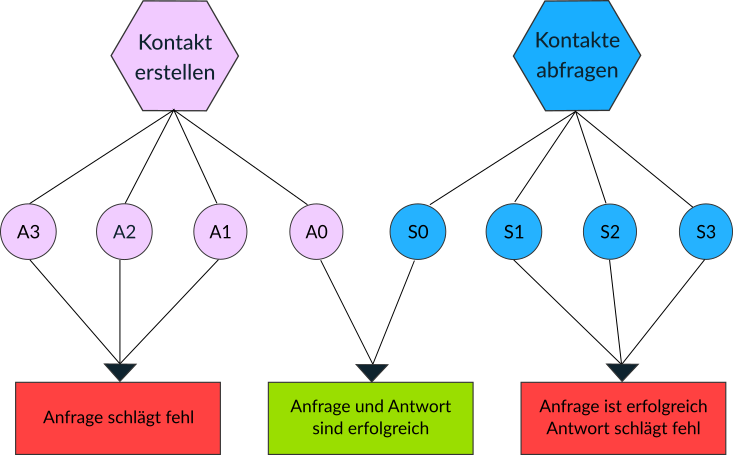
\includegraphics[width=\textwidth]{Szenarien}
\grayRule
    \caption{Use-Case-Diagramm}
    \label{fig:uc}
\end{figure}